\documentclass{beamer}
\usepackage{graphicx}
\usetheme{Madrid}
\usecolortheme{default}

\title[SAE Interpretation]
{DRP}

\subtitle{Machine Learning DRP Presentation}

\author[TODO et al.]
{TODO\inst{1} \and TODO\inst{2} \and TODO\inst{3} \and
TODO \inst{4} \and TODO \inst{5}}

\institute[UofT]
{
    \inst{1}Department of Computer Science\\
    \inst{2}Department of Statistics\\
    \inst{3}Department of Mathematics\\
    \inst{4}Department of Electrical Engineering\\
    \inst{5}Department of Cognitive Science\\
    University of Toronto
}

\date[May 2025]
{May 2025}

\logo{\includegraphics[height=0.8cm]{logo_uoft}}

\definecolor{uoftblue}{RGB}{6,41,88}
\setbeamercolor{titlelike}{bg=uoftblue}
\setbeamerfont{title}{series=\bfseries}

\begin{document}

\frame{\titlepage}

\begin{frame}
\frametitle{Table of Contents}
\tableofcontents
\end{frame}

\section{Introduction}
\begin{frame}
\frametitle{Introduction}
\begin{itemize}
    \item They describe LLMs as black boxes with \alert{billions} of uninterpretable features
    \item Sparse Autoencoders (SAEs): 
    \begin{itemize}
        \item Transform dense activations → sparse latents
        \item 1M+ features need interpretation
    \end{itemize}
    \item Manual analysis → \alert{impossible} at scale
\end{itemize}

\begin{block}{Paper's Goal/Contribution}
\begin{itemize}
    \item Automated process/pipeline for SAE latent interpretation
    \item 5 new scoring metrics
    \item Open-source code + 1M+ interpretations
\end{itemize}
\end{block}
\end{frame}


% MARIA STARTS HERE


\section{Transformers}
\begin{frame}
\frametitle{Prerequisite Vocabulary: Transformers for Text Processing}
\begin{itemize}
    \item \textbf{Tokens}: basic unit of text processed by transformers. Can be words, subwords, or characters.
    \item \textbf{Embeddings}: map tokens to dense vectors in a high-dimensional space. These vectors capture semantic relationships: similar tokens (e.g., "king" and "queen") have similar vectors.
    \begin{itemize}
        \item Embeddings turn discrete tokens into continuous vectors, allowing mathematical operations (e.g., king - man + woman = queen).
    \end{itemize}
    \item \textbf{Positional encoding}: encoding the position of each token in a sentence with a sinusoidal function. Added to the embeddings. Allows the model to learn relative positions of tokens.
\end{itemize}
\end{frame}

\begin{frame}
\frametitle{Attention is All You Need}
\begin{itemize}
    \item "Attention is All You Need" (Vaswani et al, 2017) introduced the Transformer architecture.
    \item Attention is a mathematical function defined as:\\
    $ \text{Attention}(Q, K, V) = \text{softmax}\left( \frac{QK^\top}{\sqrt{d_k}} \right) V $, where
    \begin{itemize}
        \item $Q$: Queries matrix. Identifies what a token seeks.
        \item $K$: Keys matrix. Identifies what a token offers.
        \item $V$: Values matrix. Carries the actual information to aggregate based on attention weights
        \item $d_k$: Dimension of keys (scaling prevents gradient saturation)
    \end{itemize}
    \item $Q, K, V$: learned projections 
    \item Each query vector $q_i$ computes cosine similarity with all keys $k_j$, creating attention weights that linearly combine value vectors $v_j$.
\end{itemize}
\end{frame}

\begin{frame}
\frametitle{Transformer Architecture}
\begin{figure}[h]
    \centering
    \includegraphics[width=0.8\textwidth]{transformer.png}
    \caption{Transformer architecture.}
    \label{fig:transformer}
\end{figure}
\end{frame}

\begin{frame}
    \frametitle{Attention is All You Need}
    \begin{itemize}
    \item Instead of one attention function, transformers use h=8 parallel heads:\\
        $MultiHead(Q, K, V) = MultiHead(XW_i^Q, XW_i^K, XW_i^V) = Concat(head_1, \dots, head_k)W^0$
    \item Each head applies attention to linearly projected versions of $Q, K, V$:\\
        $head_i = Attention(XW_i^Q, XW_i^K, XW_i^V)$, where $W_i^Q, W_i^K, W_i^V$ are learnable projection matrices.
    \item Each head learns a unique 'lens' to focus on different relationships (e.g., syntax vs. semantics).
    \end{itemize}
\end{frame}

\begin{frame}
    \frametitle{Our project: Interpretability}
    \textbf{Mechanistic interpretability}: understanding the internal workings of AI models by identifiying the specific mechanisms driving their behaviour.
    Why study internal model representations?
    \begin{itemize}
        \item Trust and safety: Transformers are ``black boxes". Learning how knowledge is represented in them helps build trust.
        \item Model debugging: Understanding attention patterns reveals how models prioritize features.
        \item Regulation compliance: Laws (like the EU AI Act) often require explanations for automated decisions. Interpretable transformers enable compliance in sectors like healthcare or finance.
    \end{itemize}
\end{frame}

% KIARASH STARTS HERE
\section{Sparse Autoencoders}

\begin{frame}
\frametitle{Sparse Autoencoders: Intuitive Introduction}
\begin{itemize}
    \item Transformers are powerful but as previously mentioned, they act like ``black boxes" so we need to peek inside to understand them.
    \item Sparse Autoencoders (SAEs) reveal key features the model uses by focusing on sparse and meaningful patterns in its activations.
    \item Imagine a night before your exam you're trying to memorize the whole textbook. You might highlight key sentences and ignore the rest. This is similar to how SAEs work (please don't be like SAEs in real life, the question you think can't possibly appear on your exam \textit{may} still appear). I tend to be more like SAEs :)
\end{itemize}
\end{frame}

\begin{frame}
\frametitle{Mathematical Formulation of SAEs}
\begin{itemize}
    \item An SAE has two parts: an encoder and a decoder.
    \item Encoder: Maps input $\mathbf{x} \in \mathbb{R}^n$ to a latent space $\mathbf{z} \in \mathbb{R}^m$ (where $m > n$).
    \item Decoder: Reconstructs $\hat{\mathbf{x}} \in \mathbb{R}^n$ from $\mathbf{z}$.
    \item Loss function:
    \[
    L = \| \mathbf{x} - \hat{\mathbf{x}} \|_2^2 + \lambda \| \mathbf{z} \|_1
    \]
    \item First term: Ensures $\hat{\mathbf{x}}$ matches $\mathbf{x}$ (reconstruction).
    \item Second term: Enforces sparsity in $\mathbf{z}$ using the L1 norm, controlled by $\lambda$.
    \item \textbf{Intuition: The SAE learns to represent the input with a few active features (sparse representation) while still being able to reconstruct the input.}
\end{itemize}
\end{frame}

\begin{frame}
\frametitle{Metrics for Analyzing SAEs}
\begin{itemize}
    \item \textbf{Reconstruction Error}: How well does the SAE rebuild the input? Measured with mean squared error (MSE). This is the first term in the loss function.
    \item \textbf{Sparsity}: How few features are active? Often tracked with the L1 norm or count of non-zero elements. This is the second term in the loss function.
    \item \textbf{Monosemanticity}: Do features represent single concepts? Assessed via correlation or human evaluation. This is a new metric introduced in the paper.
    \item \textbf{Interpretability}: How well can we understand the features? This is the main focus of the paper.
    \item The paper adds five new metrics for auto-interpretation (will be specified with paper details later).

\end{itemize}
\end{frame}

\begin{frame}
\frametitle{Examples of Auto-Interpreted Latents}
\begin{itemize}
    \item In language models, SAEs might find features like ``dog," ``sarcasm," or ``positive sentiment."
    \item In vision models, features could be ``red circles" or ``edges."
    \item Paper: ``Rethinking Evaluation of Sparse Autoencoders" \textcolor{blue!80}{\href{https://www.researchgate.net/publication/387975553_Rethinking_Evaluation_of_Sparse_Autoencoders_through_the_Representation_of_Polysemous_Words}{[Source]}}
\end{itemize}
\begin{figure}
    \centering
    \includegraphics[width=0.85\textwidth]{SAE3.png}
    \caption{Example of SAE-identified features in an auto-interpretability pipeline.}
\end{figure}
\end{frame}

\begin{frame}
\frametitle{Automatically Interpreting Millions of Features}
\begin{itemize}
    \item Paper Title: ``Automatically Interpreting Millions of Features in Large Language Models."
    \item Tackles interpreting SAEs at scale with:
    \begin{itemize}
        \item An automated pipeline to label SAE latents.
        \item Five new scoring metrics to judge interpretation quality.
        \item Open-source code and 1M+ feature interpretations.
    \end{itemize}
    \item Figure for the pipeline/results:
\end{itemize}
\begin{figure}
    \centering
        \includegraphics[width=0.5\textwidth]{SAE1.png}
            \caption{Automated interpretation pipeline. \textcolor{blue!80}{\href{https://arxiv.org/pdf/2410.13928}{[Source]}}}
\end{figure}
\end{frame}
    

% KIARASH ENDS HERE

% DANIEL STARTS HERE
\section{Contributions}

\begin{frame}
    \frametitle{Unanswered Questions}
    \begin{itemize}
        \item Results demonstrate similar performance between the variants, but still some important differences.
        \begin{itemize}
            \item SAE weights are different between the variants (sp. randomized vs. trained weights).
            \item Greater abstraction (as measured by entropy) in the trained weights.
            \item Feature explanations differ between the variants.
        \end{itemize}
    \end{itemize}
\end{frame}
\begin{frame}
\frametitle{Our Idea: Training as we train}
\begin{itemize}
    \item \textbf{Goal}: Current work looked at the start and end of training, we examine the stages in between.
    \item \textbf{Hypotheses}:
        \begin{itemize}
            \item The same metrics that were unable to distinguish between artifacts and real features, should display similar behavior over training checkpoints.
            \item Superposition of input data is preserved by weight checkpoints.
            \item Greater abstraction should be observed over training.
        \end{itemize}
\end{itemize}
\begin{figure}
    \centering
        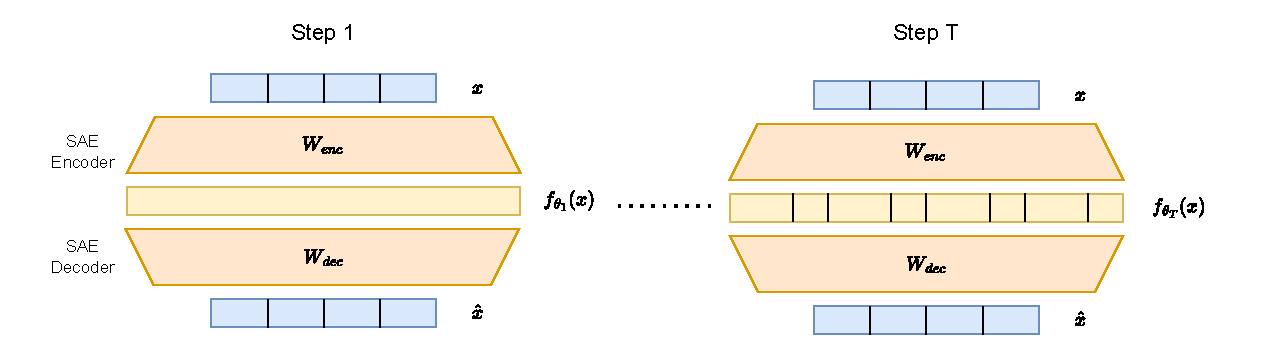
\includegraphics[width=0.7\textwidth]{training.pdf}
        \caption{Training as we train. Our implementation is based on the \textit{sparsify} package by EleutherAI. \textcolor{blue!80}{\href{
            https://github.com/EleutherAI/sparsify}{[Source]}}}
        \label{fig:training}
\end{figure}
\end{frame}

\begin{frame}
\frametitle{Dynamical Embeddings (ongoing work)}
\begin{itemize}
    \item Currently, we require training SAEs on all layers at each checkpoint.
    \item Idea is to use gradient updates on model weights to evolve the activation embeddings.
    \item Formally, if $A(t) \in \mathbb{R}^{B \times D}$ is a layer activation batch at training iteration $t$; let $Z(t) = \mathrm{Embed}(A(t)) \in \mathbb{R}^{B \times d}$ be the embedding of the activations ($d \ll D$). We want an expression \[
    Z(t + \Delta t) = \mathrm{Embed}(A(t + \Delta t)) = \mathrm{Embed}\left(A(t) - \frac{\partial \mathcal L}{\partial A(t)} \Delta t\right)
    \]
    \item This can be done if we use principal component analysis (PCA) to find the embedding of the activations.
\end{itemize}
\end{frame}

\section{Conclusion}
\begin{frame}
\frametitle{Conclusion Summary}
\begin{itemize}
    \item 5 New Scoring Metrics:
    \begin{itemize}
        \item Detection, Fuzzing, Surprisal, Embedding, Intervention
    \end{itemize}
    
    \item Important Results:
    \begin{itemize}
        \item Fuzzing: 0.69 correlation with human eval
        \item Intervention: -0.37 correlation with context scores
        \item Layer 32: 40\% higher scores than Layer 1
    \end{itemize}
    
    \item Cost Analysis:
    \begin{itemize}
        \item Embedding: \$50/100k latents
        \item Simulation: 30x more expensive
    \end{itemize}
\end{itemize}

\begin{alertblock}
{Conclusion Takeaways}
\begin{itemize}
    \item Automated interpretations help and enable SAE debugging!
    \item Output features need causal metrics
\end{itemize}
\end{alertblock}
\end{frame}

\end{document}